% vim: set spell spelllang=es syntax=tex :

En este capítulo comenzaremos analizando las estrategias de paralelización
disponibles y justificaremos la selección de las aplicadas. Esto nos permitirá
establecer las distintas tareas que ejecutará el framework y cómo se dividirán
los datos. Finalmente, una vez establecida la estructura del sistema, se
tratarán los detalles de la implementación.

\section{Discusión de las estrategias de paralelización}

\label{descripcionSistema}

Para aumentar el throughput del sistema se pueden aplicar uno o más de los
siguientes cuatro enfoques:

\begin{itemize}

	\item	Dado que en un video ya decodificado el procesamiento de cada
		cuadro es independiente del procesamiento de los demás, y dada
		la disponibilidad de recursos de cómputo, se pueden procesar
		múltiples cuadros al mismo tiempo sin que esto genere
		diferencias en la información obtenida (salvo por el orden).
		Esto permitiría aumentar la cantidad de cuadros por segundo
		obtenidos, aunque el tiempo de procesamiento de cada uno se
		mantenga igual.

	\item	Cada cuadro puede ser dividido en regiones o zonas. Esto
		permitirá realizar la búsqueda de objetos en cada zona, en
		paralelo.
		Para el correcto funcionamiento, las zonas deberán
		tener partes en común cuyos tamaños dependerán del tamaño de los
		objetos (en este caso, los robots), ya que no debe suceder que
		un objeto no aparezca completo en ninguna de las zonas. Esta
		estrategia busca reducir el tiempo de procesamiento por cuadro
		mediante el uso de múltiples unidades de procesamiento abocadas
		al mismo cuadro. Además, esta estrategia podría sacar provecho
		de una mayor localidad espacial.

	\item	Ya que la búsqueda de cada tipo de objetos es independiente de
		la búsqueda de los demás tipos, se pueden realizar múltiples
		búsquedas en paralelo sobre el mismo cuadro por cada tipo de
		objeto.

	\item	Se puede resolver el problema optimizando cada uno de los
		plugins del framework, esperando de esta manera que el tiempo de
		procesamiento de cada cuadro se reduzca lo suficiente como para
		que el sistema pueda procesar la mayoría de los cuadros a
		tiempo. Las optimizaciones pueden ser de distintos tipos, ya sea
		aplicando mejoras algorítmicas, dependientes de la arquitectura,
		aplicación de paralelismo a nivel de instrucción, etc.

\end{itemize}

Lamentablemente este último enfoque dificulta su uso como herramienta didáctica,
ya que cada plugin que se agregue o modifique deberá ser optimizado, y la
optimización puede tener impacto negativo en la legibilidad y portabilidad del
código. El primer y segundo enfoque permiten agregar y modificar los plugins sin
mayores dificultades, y en el caso en el cual un plugin no cumpla con las
condiciones que permitan aplicar alguno de los enfoques, se puede limitar el
paralelismo ya sea no dividiendo el cuadro o procesando sólo uno por vez.

Si bien el tercer enfoque también permitiría agregar o modificar los plugins
fácilmente, en las pruebas efectuadas se comprobó que realizar las búsquedas por
cada tipo de objeto en paralelo sobre cada fragmento tenía un efecto adverso.
Por este motivo, el tercer enfoque no fue aplicado sobre el producto final, y no
será incluido en las explicaciones siguientes. Los detalles de los resultados
que llevaron a tomar esta decisión serán explayados más adelante en la sección
de resultados.

\section{Tareas del sistema}

El sistema ejecuta tareas estáticas y tareas dinámicas. Las tareas estáticas son
aquellas que permanecen en ejecución desde el inicio del programa hasta su
finalización. Las tareas dinámicas son creadas para procesar un cuadro o
fragmento específico y una vez que terminan de procesar el cuadro o fragmento
finalizan. Como las tareas dinámicas son aquellas que realizan el procesamiento
para la búsqueda de los objetos, las llamamos ``tareas de búsqueda''.

Según su funcionalidad, las tareas son clasificadas en cuatro tipos:

\begin{description}

	\item[Generación de cuadros:] Es la tarea encargada de la generación o
		captura de los cuadros y colocarlos en la cola de cuadros a
		procesar. Ésta es una tarea estática, y sólo hay una en el
		sistema.

	\item[Generación de tareas de fragmentación de cuadro:] Esta tarea crea
		una tarea de fragmentación de cuadro para cada cuadro en la
		cola. Sólo toma un cuadro de la cola si hay hilos de ejecución
		para tareas de búsqueda libres. Ésta es una tarea estática, y
		sólo hay una en el sistema.

	\item[Fragmentación de cuadro:] Cada tarea de este tipo divide su cuadro
		en una cantidad predefinida de fragmentos de igual (o similar)
		tamaño. Luego, por cada fragmento, se crea una tarea de
		procesamiento de fragmento. Éstas son tareas de búsqueda, y
		puede haber múltiples en el sistema.

	\item[Procesamiento de fragmento:] Cada una de estas tareas toma su
		fragmento asociado y lo procesa utilizando cada una de las pilas
		de plugins. Éstas son tareas de búsqueda, y puede haber
		múltiples en el sistema.

\end{description}

\begin{figure}[!htb]

	\centering

	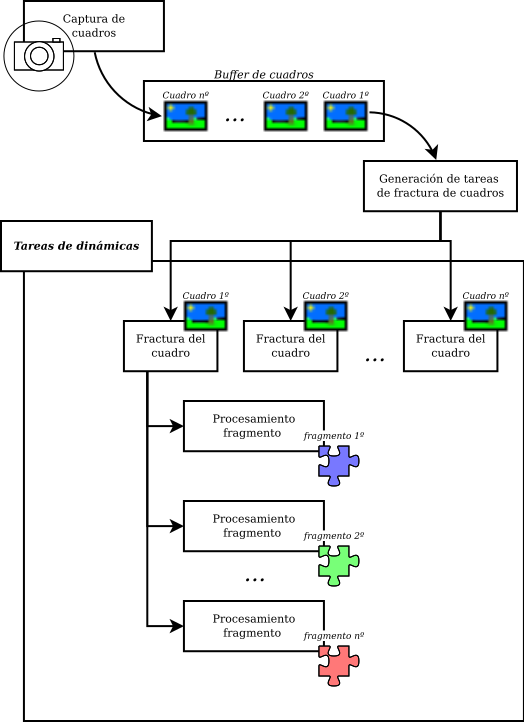
\includegraphics[height=0.45\textheight]{img/framework.pdf}

	\caption{Tareas principales del framework.}

	\label{tareasFramework}

\end{figure}

Cada una de las dos tareas estáticas tiene un hilo de ejecución asignado. Las
tareas de búsqueda son ejecutadas por un conjunto de $N$ hilos de
ejecución\footnote{$N$ es un parámetro de entrada del programa.}. Cuando un hilo
de ejecución (del conjunto) está libre, toma una nueva tarea de búsqueda para
ejecutar. Como estos hilos de ejecución son los que ejecutan las tareas de
búsqueda, nos referiremos a ellos como ``hilos de búsqueda''. En la figura
\ref{tareasFramework} se muestran un diagrama de las tareas del framework, y en
la figura \ref{hilosFramework} se muestra cómo las tareas son asignadas a los
hilos de ejecución.

La cantidad de hilos de ejecución del sistema es igual a la cantidad de hilos de
búsqueda más los dos hilos para tareas estáticas (generación de cuadros y
generación de tareas de fragmentación de cuadro). Por esto la cantidad de
unidades de procesamiento aprovechables está principalmente determinado por la
cantidad de hilos de búsqueda.

\begin{figure}[!htb]

	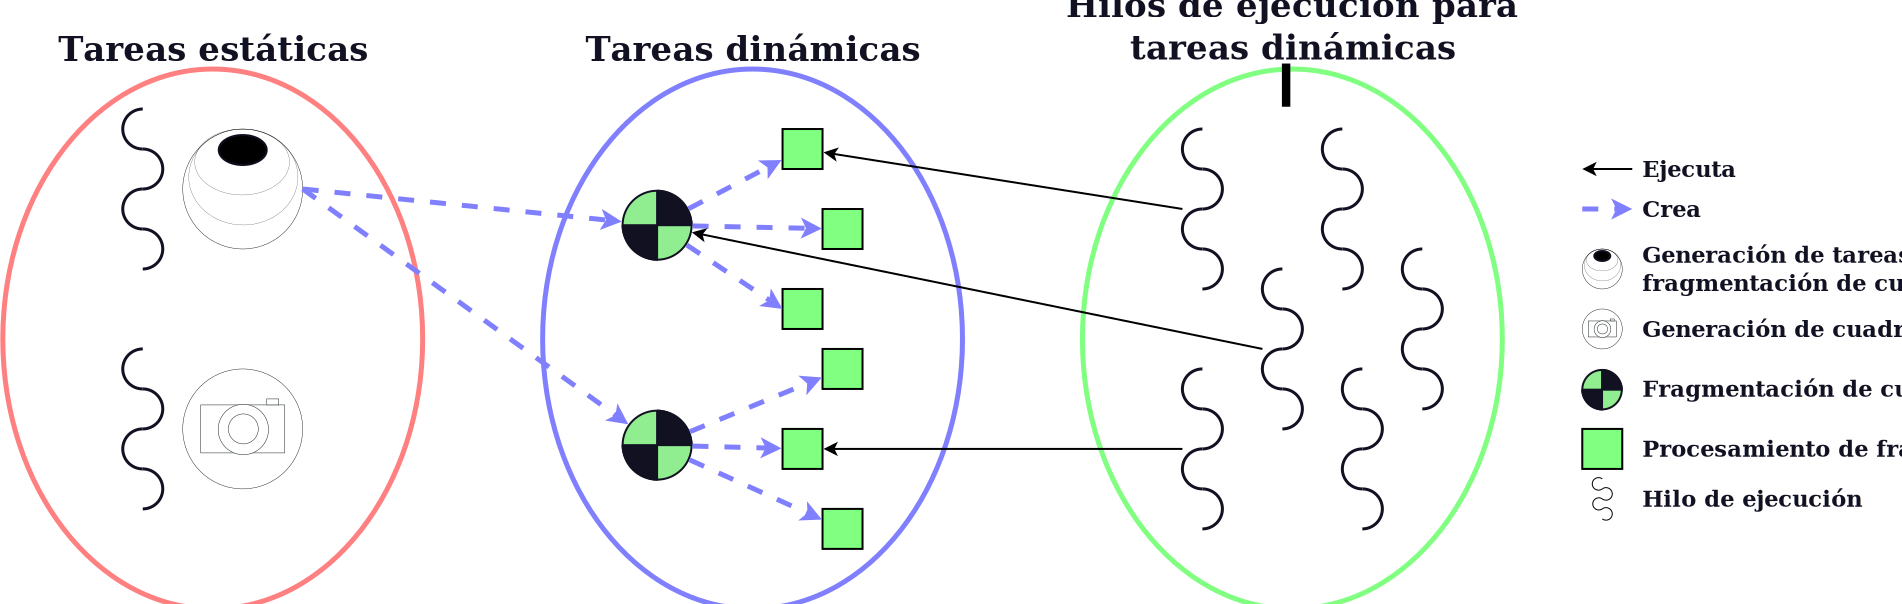
\includegraphics[width=\textwidth]{img/hilos.pdf}

	\caption{Asignación de tareas a los hilos de ejecución.}

	\label{hilosFramework}

\end{figure}

\section{Fragmentación del conjunto de datos}

Para poder realizar el procesamiento paralelo, el conjunto de datos debe ser
fragmentado; en el caso del framework propuesto la división se realizará en
dos niveles. Dado que el conjunto de datos es un video, la primera
fragmentación consta de la separación en cuadros. Como cada cuadro es una
captura del ambiente completo en un instante de tiempo específico distinto al de
los demás cuadros, se pueden procesar de forma independiente. La segunda
fragmentación de los datos se realiza dentro de cada cuadro. Ya que fragmentos
de un mismo cuadro contienen información distinta del ambiente sobre el mismo
instante, los fragmentos son dependientes entre sí. Es por eso que se deben
tener consideraciones especiales para la división del cuadro.

Si el cuadro se divide en partes sin zonas solapadas puede suceder que los
parches de un robot se encuentren en fragmentos distintos. Esto es un problema,
ya que para encontrar los robots, el plugin de detección de robots debe detectar
todos los parches que lo identifican, por lo cual todos deben estar dentro del
mismo fragmento. Para asegurar esto, cada par de fragmentos adyacentes deben
compartir una zona igual al diámetro de un robot. En la figura
\ref{areaCompartida} se muestran los casos donde el área compartida es menor al
diámetro de un robot y donde el área compartida es del diámetro de un robot.

\begin{figure}[!htb]

	\centering
	
\includegraphics[width=0.45\textwidth]{img/areaTooSmall.pdf}
	
\includegraphics[width=0.45\textwidth]{img/areaPerfect.pdf}

	\caption{Izquierda: si el área compartida es demasiado pequeña y si el
	robot se encuentra entre dos fragmentos, puede que sus parches no sean
	completamente visibles desde ninguno de ellos. Derecha: si el área
	compartida es del ancho de los robots, entonces todos los parches son
	visibles completamente desde por lo menos un fragmento.}

	\label{areaCompartida}

\end{figure}

Dado que los fragmentos comparten una área en sus bordes, la suma del área de
los fragmentos es superior al área de la imagen original. Para reducir los
píxeles a procesar, se debe reducir la zona compartida. Como la zona compartida
tiene un ancho fijo (el diámetro de un robot), para encontrar el área compartida
mínima se debe minimizar el perímetro del fragmento.

Por la manera que las imágenes se representan comúnmente en una computadora y
por su simplicidad, se optó por trabajar con un teselado con rectángulos. En el
caso de éstos, para minimizar su perímetro y maximizar su área, se debe procurar
que la relación entre su ancho y alto sea lo más cercana posible a uno.
También, para balancear la carga uniformemente, todos los fragmentos serán de
igual tamaño.

El tiempo de procesamiento de un fragmento depende no sólo de su área, sino que
es influido por los elementos encontrados por los plugins, por lo cual
fragmentos de igual tamaño pueden tener tiempos de procesamiento muy distintos.
Esta información puede ser inferida utilizando la información de cuadros
anteriores, sin embargo esto viola la independencia entre cuadros. Por esto, la
heurística que se utiliza para distribuir la carga de procesamiento es que todos
los fragmentos sean de igual tamaño. Aquellos que se encuentren en los bordes
inferior y derecho posiblemente serán más pequeños, ya que las dimensiones del
cuadro pueden no ser divisibles por el número de columnas o filas en las cuales
se dividirá.

En la figura \ref{fragmentos} se muestran como se divide un cuadro de 800x600
píxeles con un área compartida de 50 píxeles en 1, 2, 5 y 8 fragmentos. Cuando
el número de fragmentos es un número primo, como en el caso de 5 fragmentos, el
cuadro se divide en franjas de igual ancho o alto que el cuadro original. Este
tipo de división produce fragmentos con perímetros mayores, produciendo grandes
áreas compartidas.

\begin{figure}[!htb]

	
\includegraphics[width=0.5\textwidth]{img/fragmentos1.pdf}
	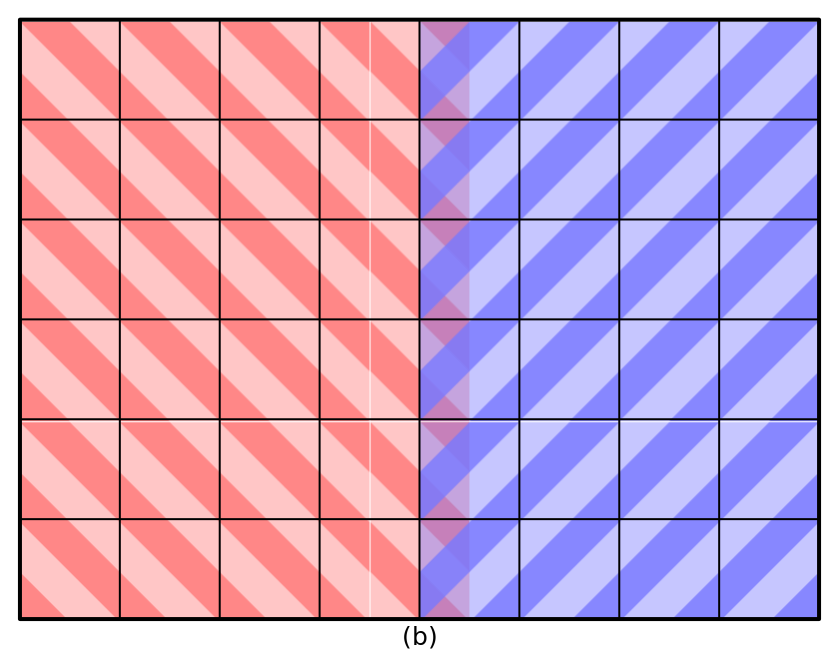
\includegraphics[width=0.5\textwidth]{img/fragmentos2.pdf}
	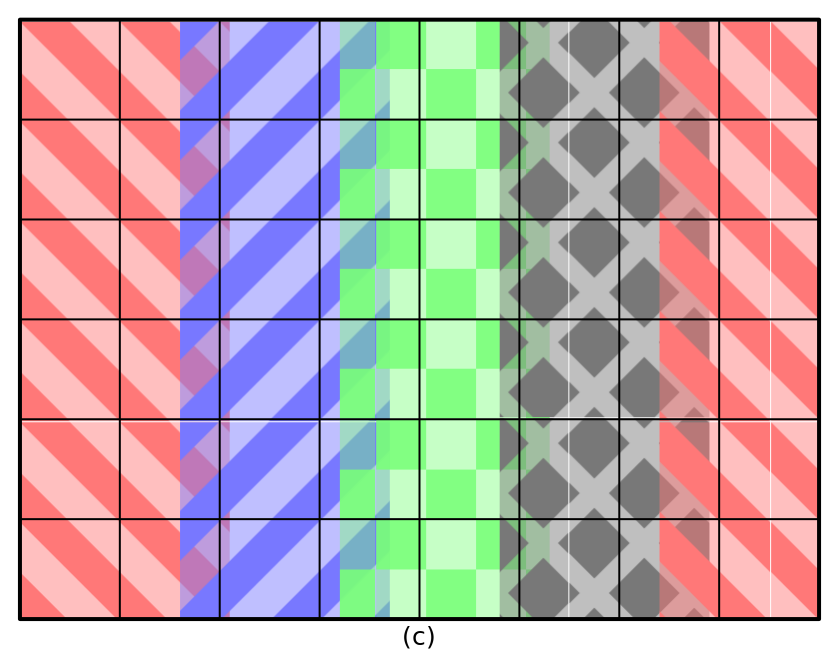
\includegraphics[width=0.5\textwidth]{img/fragmentos5.pdf}
	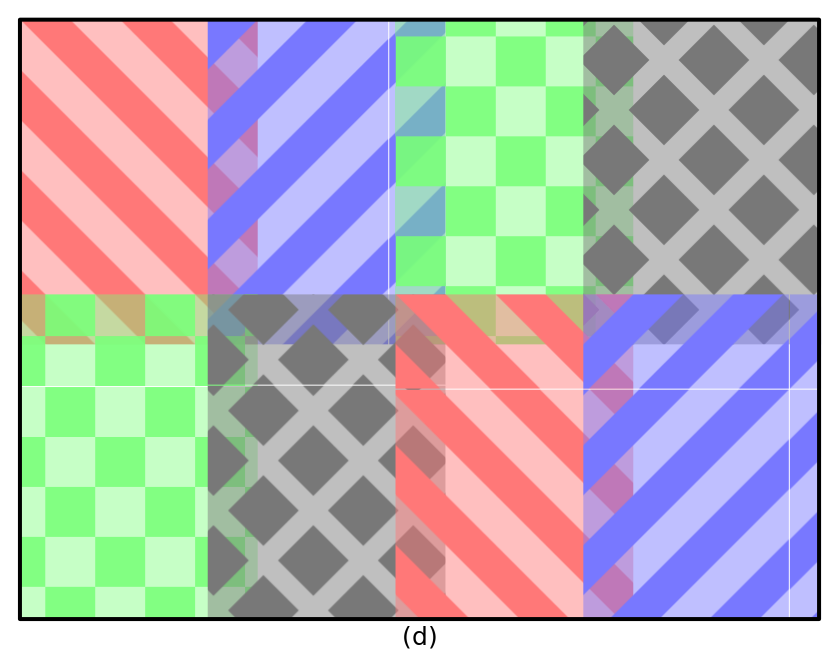
\includegraphics[width=0.5\textwidth]{img/fragmentos8.pdf}
	\caption{Resultado de dividir un cuadro de 800x600 píxeles con un área
	compartida de 50 píxeles en 1(a), 2(b), 5(c) y 8(d) fragmentos.}
	\label{fragmentos}

\end{figure}

\section{Implementación del framework}

\label{implementacionFramework}

Como primera etapa se implementó un framework base que simula el procesamiento de
ítems prototipo vacíos y establece las clases base a ser extendidas. Esto
permite explicar el flujo de la información así como la estructura base del
sistema sin preocuparse por la implementación específica para el sistema de
visión global para el fútbol de robots.

El framework fue implementado en \emph{C++} con \emph{OpenMP} y está basado en
plugins para facilitar su modificación en un ambiente educativo. La elección del
lenguaje se debe principalmente a su eficiencia e implementación del paradigma
orientado a objetos. Dado que el sistema debe procesar los cuadros en tiempos
acotados, la eficiencia es crucial, mientras que el paradigma orientado a
objetos permite establecer fácilmente la interfaz de los plugins. El uso de
\emph{OpenMP} permite la creación y control de hilos de ejecución y tareas de
forma sencilla.  Se utilizaron los plugins implementados en \cite{torres2014},
modificándolos para permitir su uso en un sistema paralelo.

En la figura \ref{codigo} se muestra el fragmento de código (en pseudocódigo)
que ejecuta y crea las tareas principales del framework. En la función principal
(\emph{main}, línea 1 a 19) se crean las tareas de generación de cuadros (líneas
6 y 7) y generación de tareas de fragmentación de cuadros (líneas 8 a 10)
utilizando el modelo de \emph{fork and join}. El control de la finalización del
programa se realiza a través de una variable compartida \emph{continuar}.

La tarea de generación de tareas de fragmentación de cuadros se implementa en la
función \emph{generaciónDeTareasDeFragmentaciónDeCuadros} (líneas 23 a 58). La
función comienza estableciendo una región de trabajo compartido bajo el modelo
de tareas. Se crean $N+1$ hilos de ejecución (línea 25), $N$ hilos para las
tareas de búsqueda y uno adicional para la tarea de generación de tarea de
fragmentación de cuadros. La tarea de generación de tareas de fragmentación de
cuadros implementa una espera ocupada sobre la cola de cuadros a procesar. La
finalización de la tarea es controlada por la variable \emph{continuar}.

Cuando hay hilos de búsqueda libres y cuadros en la cola de cuadros, se toma un
cuadro de la cola de cuadros (líneas 29 a 32), y se crea una tarea de
fragmentación de cuadro con una copia privada del puntero al cuadro (líneas 33 a
36).

Cada tarea de fragmentación de cuadro (líneas 37 a 53), comienza fragmentando el
cuadro. Por cada fragmento crea una tarea de procesamiento de fragmento (líneas
40 a 43). Cuando la tarea de fragmentación de cuadro finaliza, libera al hilo de
ejecución.

Cada tarea de procesamiento de fragmento (líneas 44 a 52) procesa el fragmento
con cada pila (líneas 45 a 48). Cuando se termina de procesar el fragmento con
todas las pilas se borra el fragmento (línea 49) y se libera el hilo de
ejecución.

\begin{figure}[!htb]

	\centering

	\includegraphics[width=0.5\textheight]{img/itemSwitch.pdf}

	\caption{Pseudo código del sistema}

	\label{codigo}

\end{figure}

En la figura \ref{hilosytareas} se muestra una posible secuencia de ejecución.
Dado que el procesamiento de los fragmentos tiene un tiempo variable, los hilos
se liberan de forma irregular, lo que lleva a que el orden de creación de las
tareas para los distintos cuadros no sea completamente determinista.

\begin{figure}[!htb]

	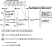
\includegraphics[width=\textwidth]{img/hilosytareas.pdf}

	\caption{Asignación de las tareas a los hilos de búsqueda}

	\label{hilosytareas}

\end{figure}

Las clases del framework básico son las siguientes:

\begin{description}

	\item[Item:] Esta clase define un tipo prototipo de los ítems que serán
		tratados por el sistema. En la implementación específica para el
		sistema de visión global para el fútbol de robots, los cuadros
		son subclase de la clase \emph{Item}.

	\item[RingBuffer:] Éste es el buffer donde se guardan los ítems
		generados mientras esperan ser procesados. El buffer guarda sólo
		punteros a objetos de la clase \emph{Item} y no tiene mecanismos
		de control que permitan acceder la estructura desde múltiples
		hilos al mismo tiempo de forma segura. Cuando se solicita un
		ítem, se devuelve el puntero al más antiguo o \textbf{NULL} en
		caso de que la estructura esté vacía. Cuando se intenta agregar
		un nuevo ítem pero la estructura está llena, se coloca éste en
		el espacio del ítem más viejo en la estructura y se retorna el
		puntero de éste al llamador, delegándole su destrucción. La
		razón de la delegación de la destrucción se debe a que la
		destrucción un objeto es lenta (y aun mayor en el caso de los
		cuadros del sistema final), y el control de acceso al buffer se
		realiza a través del uso de de secciones críticas, por lo que es
		importante reducir el tiempo que cada hilo pasa dentro de la
		sección crítica, para no impedirle el acceso a otros hilos que
		pueden estar esperando entrar a ellas.

	\item[Input:] Se trata de una clase que funciona como definición de la
		interfaz de las clases que generan los ítems. Sus métodos
		principales son \emph{run} y \emph{generate}. El método
		\emph{generate} debe ser reimplementado por las clases hijas
		para generar el tipo de ítem especifico del sistema. El método
		\emph{run} es el encargado de generar los ítems llamando a
		\emph{generate} y colocarlos en el \emph{RingBuffer}. Este
		último método puede ser redefinido si la aplicación así lo
		requiere.

	\item[ItemSlicer:] Es la clase que define la interfaz de las clases
		encargadas de dividir los ítems. Se definen tres métodos. El
		primero es \emph{slice} que recibe como parámetro un ítem y la
		cantidad de partes en la que éste debe ser dividido y retorna un
		arreglo de ítems. Algunos plugins pueden agregar información a
		los fragmentos de los ítems, con el fin de ser utilizada por
		plugins posteriores dentro de la misma pila, es por esto que
		antes de continuar con la siguiente pila se utiliza el método
		\emph{resetItem} que elimina la información agregada por los
		plugins, retornando al fragmento a su configuración inicial. El
		tercer método es \emph{delPart} que recibe como parámetro un
		fragmento de ítem y lo elimina.

	\item[Plugin:] Esta clase define una interfaz para los plugins que
		realizarán las distintas partes del procesamiento de la imagen.
		Sólo se define el método \emph{process} que tiene como único
		parámetro un puntero a un objeto de la clase \emph{Item}.

	\item[PluginStack:] Ésta es la clase que tomará el ítem y se encargará
		de entregarlo a cada uno de los plugins. Tiene sólo dos métodos,
		\emph{addPlugin}, para agregar un plugin, y \emph{process} que
		tiene como parámetro un ítem, para procesarlo.

	\item[ItemSwitch:] Ésta es la clase encargada de implementar la tarea de
		generación de tareas de fragmentación de cuadro. Para no crear
		más tareas de las que puede procesar el sistema, sólo se toma un
		cuadro de la cola de cuadros a procesar si hay hilos de búsqueda
		libres (o lo que es lo mismo, la cola de tareas está vacía).
		Cada tarea de fragmentación de cuadro divide el ítem utilizando
		\emph{ItemSlicer} y crea una nueva tarea de procesamiento de
		cuadros por cada fragmento.

\end{description}

En la figura \ref{clasesFramework} se muestra el diagrama de clases del
framework base.

\begin{figure}[!htb]

	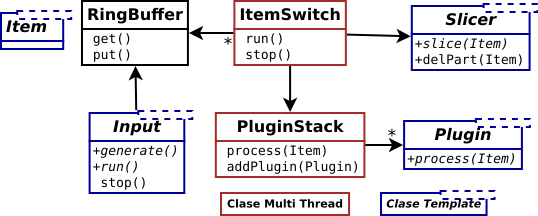
\includegraphics[width=\textwidth]{img/clasesFramework.pdf}

	\caption{Diagrama de clases Framework base.}

	\label{clasesFramework}

\end{figure}

Existen dos parámetros ajustables. El primero es la cantidad de hilos que
ejecutarán las tareas de búsqueda. El segundo parámetro es la cantidad de partes
en las cuales se dividirá el cuadro.

Para extender el framework para utilizarlo como un sistema de visión por
computadora para el fútbol de robots se incorporaron las siguientes clases, las
cuales fueron tomadas y modificadas del sistema de visión presentado en
\cite{torres2014}:

\begin{description}

	\item[Frame:] Subclase de \emph{Item}. Contiene una imagen que
		representa un cuadro y una estructura auxiliar que contiene la
		información necesaria para el funcionamiento de los plugins.

	\item[CaptureFromFile:] Subclase de \emph{Input}. Es la clase encargada
		de crear el flujo de objetos \emph{Frame}, tomando cada cuadro
		desde un archivo de video. También debe respetar la taza de
		cuadros por segundo del video.

	\item[FastCaptureFromFile:] Subclase de \emph{Input}. Muy similar a
		\emph{CaptureFromFile}, con las diferencias de que carga los
		cuadros a memoria antes de que comience el sistema a capturar
		los cuadros (para evitar los retardos de la lectura de disco y
		decodificación), y que tiene dos modos de controlar la
		frecuencia de la generación de los cuadros. Se puede adelantar
		la creación de cuadros si la cola de cuadros a procesar está
		vacía, o fijar la frecuencia de su creación a un valor
		especifico. Esta clase es útil para comprobar la capacidad
		máxima del sistema, ya que permite simular una cámara con la
		velocidad de captura que se desee, y los distintos modos
		permiten testear la carga máxima en cuadros por segundo
		soportada por el sistema, así como los tiempos de espera bajo
		una cantidad de cuadros por segundo especifica.

	\item[FrameSlicer:] Subclase de \emph{ItemSlicer}. Cada cuadro es
		dividido en rectángulos del mismo tamaño (excepto por los
		cuadros en los bordes inferior y derecho, que posiblemente sean
		más pequeños). Cada subcuadro incluye un área solapada con los
		cuadros adyacentes para asegurar que todos los objetos (robots y
		pelota) se encuentren completamente en por lo menos un
		subcuadro.

	\item[Subclases de \emph{Plugin}:] \emph{PluginBlur},
		\emph{PluginColorConversions}, \emph{PluginColorSegmentation},
		\emph{PluginDetectBalls}, \emph{PluginFindBlobs},
		\emph{PluginFindSecondariesBlobs}, \emph{PluginMorphology} y
		\emph{PluginNetworking}.

	\item[Clases auxiliares:] \emph{ball}, \emph{colorspace},
		\emph{datastruct}, \emph{homography}, \emph{marker},
		\emph{pattern}, \emph{pattern\_matching},
		\emph{practicalsocket}, \emph{segmentation}, \emph{team},
		\emph{timer}.

\end{description}

En la figura \ref{clasesFrameworkRobots} se muestra el diagrama de clases del
framework extendido para ser utilizado como sistema de visión global para
fútbol de robots.

\begin{figure}[!htb]

	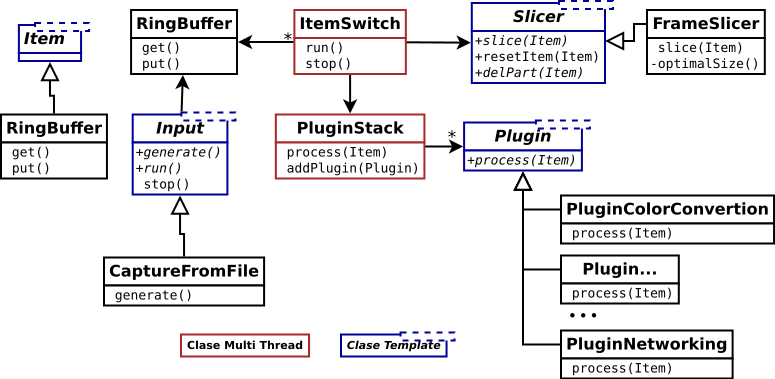
\includegraphics[width=\textwidth]{img/clasesFrameworkRobots.pdf}

	\caption{Diagrama de clases del sistema de visión para el fútbol
	de robots.}

	\label{clasesFrameworkRobots}

\end{figure}

Conceptualmente, la implementación para fútbol de robots tiene dos pilas, una
para búsqueda de robots y la otra para búsqueda de la pelota. Sin embargo, para
ambas pilas los primeros tres plugins realizan la misma tarea de
preprocesamiento (plugins de conversión de color, segmentación de color y
morfología), mientras que los plugins propios de cada pila (para la búsqueda de
la pelota: plugin de búsqueda de pelota. Para la búsqueda de los robots: plugins
de detección de regiones principales y detección de regiones secundarias) no
modifican el cuadro, permitiendo unir ambas pilas en una sola y realizar el
preprocesamiento una vez por cuadro. El plugin de difusión se ejecutará dos
veces, una para enviar los datos de la pelota y otra para enviar los datos de
los robots. En la figura \ref{pilasUnificadas} se muestra la pila de búsqueda
unificada que utiliza el sistema final.

\begin{figure}[!htb]

	\centering

	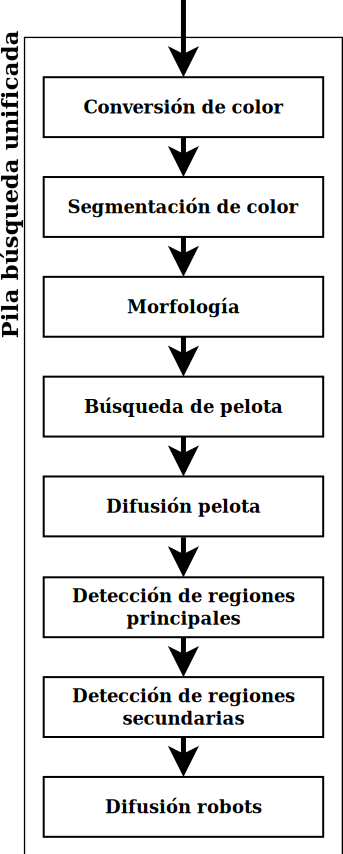
\includegraphics[height=0.45\textheight]{img/pilasUnificadas.pdf}

	\caption{Pila de búsqueda unificada utilizada por el sistema final.}

	\label{pilasUnificadas}

\end{figure}
